\باب{حدود اور استمرار}
\جزوحصہء{جائزہ}
تفاعل کی حد کا تصور ان بنیادی تصورات میں سے ایک ہے جو احصاء کو الجبرا اور تکونیات سے علیحدہ کرتا ہے۔

اس باب میں ہم حدود کے تصور کو پہلے وجدانی طور پر اور بعد میں با ضابطہ وضع کرتے ہیں۔ہم حدود کو استعمال کرتے ہوئے تفاعل \عددی{f} میں تبدیلی پر غور کرتے ہیں۔کچھ تفاعل مسلسل تبدیل ہوتے ہیں جہاں \عددی{x} میں چھوٹی تبدیلی، \عددی{f(x)} میں چھوٹی تبدیلی ہی پیدا ہوتی ہے۔دیگر تفاعل میں \عددی{x} کی چھوٹی تبدیلی، \عددی{f(x)} میں چھلانگ یا غیر یقینی تبدیلی  پیدا کر سکتی ہے۔ ہم حدود کو استعمال کرتے ہوئے تفاعل کی ترسیم کے مماثل خطوط متعارف کریں گے۔ اس جیومیٹریائی استعمال کی بنا تفاعل کی تفرق کا تصور پیدا ہو گا۔تفاعل کی تفرق، جس پر اگلے باب میں تفصیلاً غور کیا جائے گا، تفاعل کی تبدیلی کو تعین کرتا ہے۔

\حصہ{تبدیلی کی شرح اور حد}
اس حصہ میں ہم تبدیلی کی شرح کی دو مثالیں، رفتار اور نمو آبادی متعارف کرتے ہیں جن سے اس باب کا اصل موضوع، حد کا تصور پیدا ہو گا۔

\جزوحصہء{رفتار}
کسی بھی دورانیے میں متحرک جسم کی اوسط رفتار سے مراد اس وقت میں طے فاصلہ تقسیم دورانیہ ہے۔

\ابتدا{مثال}
ایک پتھر \عددی{\SI{100}{\meter}} اونچائی سے گرتا ہے۔ (الف) پہلی دو سیکنڈ میں (ب) پہلی سے دوسری سیکنڈ کے دارانیے  میں پتھر کی اوسط رفتار  کیا ہو گی؟\\
حل:\quad
ہم جانتے ہیں کہ سطح زمین کے قریب ساکن حالت سے گرتا ہوا جسم پہلی \عددی{t} سیکنڈوں میں
\begin{align*}
y=4.9 t^2
\end{align*}
میٹر فاصلہ طے کرتا ہے۔یوں پہلی \عددی{t} سیکنڈ میں اوسط رفتار جاننے کے لئے ہم فاصلہ میں تبدیلی \عددی{\Delta y} کو وقت میں تبدیلی \عددی{\Delta t} سے تقسیم کرتے ہیں۔\\
(الف)\quad
پہلی دو سیکنڈ میں اوسط رفتار
$\tfrac{\Delta y}{\Delta t}=\tfrac{4.9(2)^2-4.9(0)^2}{2-0}=\SI{9.8}{\meter\per\second}$
ہو گی۔\\
(ب)\quad 
پہلی اور دوسری سیکنڈ کے دوران اوسط رفتار
$\tfrac{\Delta y}{\Delta t}=\tfrac{4.9(2)^2-4.9(1)^2}{2-1}=\SI{14.7}{\meter\per\second}$
ہو گی۔
\انتہا{مثال}
%======================= 
\ابتدا{مثال}
پتھر کی رفتار \عددی{t=\SI{1}{\second}} اور \عددی{t=\SI{2}{\second}} پر تلاش کریں۔\\
حل:\quad
ہم وقتی وقفہ \عددی{[t_0,t_0+h]}  پر اوسط رفتار حاصل کرتے ہیں، یعنی:
\begin{align*}
\frac{\Delta y}{\Delta t}=\frac{4.9(t_0+h)^2-4.9t^2_0}{h}
\end{align*}
چونکہ کسی بھی عدد کو صفر سے تقسیم نہیں کیا جا سکتا ہے لہٰذا درج بالا کلیہ میں \عددی{h=0} پر کرتے ہوئے  "لمحاتی رفتار" حاصل نہیں کی جا سکتی ہے۔البتہ اس کلیہ کو استعمال کرتے ہوئے ہم کم سے کم  دورانیے کے لئے اوسط رفتار حاصل کر سکتے ہیں۔یوں \عددی{t_0=1} اور \عددی{t_0=2} کے لئے \عددی{h=0.1,0.01,\cdots} لیتے ہوئے  درج ذیل اوسط رفتار حاصل کیے جا سکتے ہیں۔
\begin{align*}
\begin{array}{lll}
\hline
\multicolumn{1}{c}{h}&\multicolumn{1}{c}{\text{\RL{پر اوسط رفتار}} t_0=1} &\multicolumn{1}{c}{ \text{\RL{پر اوسط رفتار}} t_0=2}\\
\hline
1&14.7&24.5\\
0.1&10.29&20.09\\
0.01&9.84899&19.64899\\
0.001&9.80489&19.60489\\
0.0001&9.800489&19.60049
\end{array}
\end{align*}
آپ دیکھ سکتے ہیں کہ \عددی{t_0=1} کے لئے \عددی{h} کی قیمت کم سے کم کرتے ہوئے اوسط رفتار \عددی{\SI{9.8}{\meter\per\second}}  کے قریب تر ہوتی جاتی ہے جس سے ہم کہہ سکتے ہیں کہ \عددی{t_0=1} پر پتھر کی رفتار \عددی{\SI{9.8}{\meter\per\second}} ہو گی۔اسی طرح \عددی{t_0=2} پر پتھر کی رفتار \عددی{\SI{19.6}{\meter\per\second}} نظر آئے گی۔
\انتہا{مثال}
%============================

\جزوحصہء{اوسط شرح تبدیلی اور سیکنٹ خطوط}
\عددی{x} کے لحاظ سے تفاعل \عددی{f(x)} کی اوسط شرح تبدیلی کو   وقفہ \عددی{[x_1,x_2]}  پر حاصل کرنے کی خاطر ہم \عددی{y} کی قیمت میں تبدیلی،
 \عددی{\Delta y=f(x_2)-f(x_1)} کو \عددی{x} کی قیمت میں تبدیلی \عددی{\Delta x=x_2-x_1=h} سے تقسیم کرتے ہیں۔

\ابتدا{تعریف}
\عددی{x} کے لحاظ سے وقفہ \عددی{[x_1,x_2]} پر \عددی{y=f(x)} کی اوسط شرح تبدیلی درج ذیل ہو گی۔
\begin{align*}
\frac{\Delta y}{\Delta x}=\frac{f(x_2)-f(x_1)}{x_2-x_1}=\frac{f(x_1+h)-f(x_1)}{h}
\end{align*}
\انتہا{تعریف}
%=====================

آپ دیکھ سکتے ہیں کہ وقفہ \عددی{[x_1,x_2]} پر \عددی{f} کی اوسط شرح تبدیلی نقطہ \عددی{N(x_1,f(x_1))} اور نقطہ \عددی{Q(x_2,f(x_2))} سے گزرتے ہوئے خط کی ڈھلوان کے برابر ہے (شکل \حوالہ{شکل_حد_سیکنٹ_ڈھلوان})۔جیومیٹری میں ترسیم پر کسی دو نقطوں سے گرتے ہوئے خط کو ترسیم کا \اصطلاح{سیکنٹ}\فرہنگ{سیکنٹ}\حاشیہب{secant}\فرہنگ{secant} کہتے ہیں۔یوں \عددی{x_1} سے \عددی{x_2}  تک  اوسط شرح تبدیلی سیکنٹ \عددی{NQ} کی ڈھلوان کے برابر ہے۔ 
\begin{figure}
\centering
\begin{tikzpicture}[font=\small]
\draw[-latex](-0.25,0)--(5,0)node[right]{$x$};
\draw[-latex](0,-0.2)--(0,2.5)node[above]{$y$};
\draw(1.5,0.5) to [out=-10,in=-110] coordinate[pos=0.2](kA) coordinate[pos=0.75](kB)(5,2.5)node[left]{$y=f(x)$};
\draw[shorten <=-0.5cm,shorten >=-0.5cm](kA)--(kB)node[pos=0.5,sloped,above ]{سیکنٹ};
\draw(kA)node[circ,pin=135:{$N(x_1,f(x_1))$}]{} (kB)node[circ]{}node[above left]{$Q(x_2,f(x_2))$};
\draw[dashed] (kA)--($(0,0)!(kA)!(5,0)$)node[below]{$x_1$};
\draw[dashed] (kB)--($(0,0)!(kB)!(5,0)$)node[below]{$x_2$}coordinate(kC);
\draw[dashed](kA)--($(kB)!(kA)!(kC)$)coordinate(kD)node[pos=0.5,below]{$\Delta x$};
\path(kB)++(0.1,0)coordinate(kBB);
\path(kD)++(0.1,0)coordinate(kDD);
\draw[stealth-stealth] (kBB)--(kDD)node[pos=0.5,right]{$\Delta y$};
\draw(0,0)node[below left]{$M$};
\end{tikzpicture}
\caption{منحنی کی اوسط شرح تبدیلی سیکنٹ کی ڈھلوان کے برابر ہو گی۔}
\label{شکل_حد_سیکنٹ_ڈھلوان}
\end{figure}

%====================

\ابتدا{مثال}\شناخت{مثال_حد_نمو_آبادی_مکھی}\ترچھا{نمو آبادی کی اوسط شرح}\\
ایک تجربہ میں قابو ماحول میں مکھیوں کی تعداد کو \عددی{40} دن کے عرصہ پر روزانہ گنا گیا۔تعداد بالمقابل دنوں کو ترسیم کرتے ہوئے نقطوں کو ہموار منحنی سے جوڑا گیا (شکل \حوالہ{شکل_حد_مکھی_نمو_آبادی})۔  \عددی{20} ویں دن  سے  \عددی{37} ویں دن  تک آبادی کی اوسط شرح تبدیلی دریافت کریں۔\\
 \begin{figure}
\centering
\begin{minipage}{0.45\textwidth}
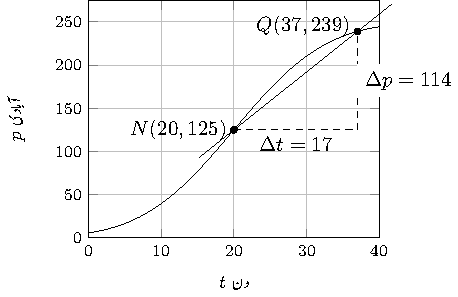
\includegraphics{normalDistributionFlies}
\caption{مکھی کی نمو آبادی}
\label{شکل_حد_مکھی_نمو_آبادی}
\end{minipage}\hfill
\begin{minipage}{0.45\textwidth}
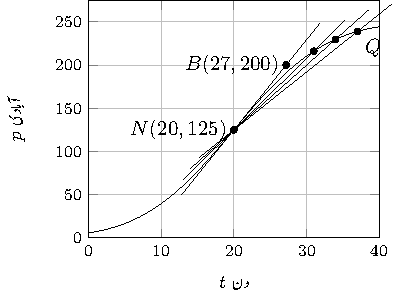
\includegraphics{normalDistributionFliesInstantaneous}
\caption{مکھی کی بیسویں دن نمو آبادی}
\label{شکل_حد_مکھی_نمو_آبادی_بیس}
\end{minipage}%
\end{figure}

حل:\quad
\عددی{20} ویں دن آبادی \عددی{125} تھی جبکہ \عددی{37} ویں دن آبادی \عددی{239} تھی۔ یوں \عددی{37-20=17} دنوں میں آبادی میں \عددی{239-125=114} تبدیل  رونما ہوئی۔یوں شرح تبدیلی درج ذیل ہو گی
\begin{align*}
\frac{\Delta p}{\Delta t}=\frac{114}{17}=6.7 (\text{\RL{مکھیاں فی دن}})
\end{align*}
جو شکل \حوالہ{شکل_حد_مکھی_نمو_آبادی} میں سیکنٹ \عددی{NQ} کی ڈھلوان ہے۔
\انتہا{مثال}
%========================

درج بالا مثال میں \عددی{20} ویں دن سے \عددی{37} ویں دن تک کی اوسط شرح تبدیلی حاصل کی گئی جو ہمیں \عددی{20} ویں دن کی تبدیلی کی شرح کے بارے میں کوئی معلومات فراہم نہیں کرتی ہے۔اس کے لئے ہمیں \عددی{20} ویں دن کے قریب حساب  کرنا ہو گا۔

\ابتدا{مثال}
مثال \حوالہ{مثال_حد_نمو_آبادی_مکھی} میں \عددی{20} ویں دن آبادی میں تبدیلی کی شرح کیا ہے؟\\
حل:\quad
ہمیں نقطہ \عددی{Q} کو نقطہ \عددی{N} کے قریب سے قریب تر کرتے ہوئے شرح حاصل کرنی ہو گی (شکل \حوالہ{شکل_حد_مکھی_نمو_آبادی_بیس})۔یوں درج ذیل حاصل ہوتا ہے۔
\begin{align*}
\begin{array}{ll}
Q&\frac{\Delta p}{\Delta t}\\
\hline
(37,239)&\frac{239-125}{37-20}=6.7\\
(35,230)&\frac{230-125}{35-20}=7\\
(32,216)&\frac{216-125}{32-20}=7.6\\
(27,200)&\frac{200-125}{27-20}=10.7
\end{array}
\end{align*}

جیسے جیسے \عددی{Q} کو بائیں منتقل کیا جائے، خط \عددی{NQ} نقطہ \عددی{N} کے گرد گھڑی کی الٹ رخ گھومتا ہے۔ہم دیکھتے ہیں کہ یہ خط آخر کار \عددی{NB} کو چھوتا ہے۔اس خط کو دیے گئے منحنی کا \اصطلاح{مماس}\فرہنگ{مماس}\حاشیہب{tangent}\فرہنگ{tangent} کہتے ہیں۔اس طرح ہم توقع کرتے ہیں کہ \عددی{20} ویں دن آبادی کی تبدیلی کی شرح \عددی{10.7} مکھیاں فی دن ہو گی۔
\انتہا{مثال}
%=======================

لمحہ \عددی{t=1} اور لمحہ \عددی{t=2} پر گرتے ہوئے پتھر کی رفتار یا \عددی{20} ویں دن شرح تبدیلی کو \اصطلاح{لمحاتی شرح تبدیلی}\فرہنگ{لمحاتی!شرح تبدیلی}\حاشیہب{instantaneous rates of change}\فرہنگ{instantaneous!rate of change} کہتے ہیں۔جیسا آپ نے دیکھا، ہم اوسط شرح تبدیلی کی تحدیدی قیمت سے لمحاتی شرح تبدیلی حاصل کرتے ہیں۔درج بالا مثال میں ہم نے خط مماس کو بطور خط سیکنٹ کی تحدیدی  صورت پیش کیا۔لمحاتی شرح اور مماس کا گہرا تعلق ہے جو دیگر موضوعات میں بھی پیش آتا ہے۔ اس تعلق کو مزید سمجھنے کی خاطر ہمیں  تحدیدی قیمتوں  کا تعین کرنا سیکھنا ہو گا جنہیں ہم \اصطلاح{حد}\فرہنگ{حد}\حاشیہب{limits}\فرہنگ{limits} کہتے ہیں۔ 

\جزوحصہء{تفاعل کی تحدیدی قیمتیں}
تحدیدی قیمت کی تعریف سے پہلی ایک اور مثال دیکھتے ہیں۔

\ابتدا{مثال}\شناخت{مثال_حد_عجیب_تفاعل_الف}
تفاعل \عددی{f(x)=\tfrac{x^2-1}{x-1}} نقطہ \عددی{x=1} کے قریب کیسا رویہ رکھتا ہے؟\\
حل:\quad
چونکہ صفر سے کسی بھی عدد کو تقسیم نہیں کیا جا سکتا ہے لہٰذا ماسوائے \عددی{x=1} کے، یہ کلیہ تمام حقیقی اعداد کے لئے \عددی{f} تعین کرتا ہے۔کسی بھی \عددی{x\ne 1} کے لئے ہم اس کلیہ کی سادہ صورت حاصل کر سکتے ہیں:
\begin{align*}
f(x)=\frac{x^2-1}{x-1}=\frac{(x-1)(x+1)}{x-1}=x+1\quad\quad (x\ne 1)
\end{align*} 
یوں خط \عددی{y=x+1} جس سے نقطہ \عددی{x=1} یعنی \عددی{(1,2)} خارج کیا گیا ہو اس تفاعل کو ظاہر کرتا ہے۔اس نقطہ کو شکل \حوالہ{شکل_مثال_حد_عجیب_تفاعل_الف} میں بطور سوراخ دکھایا گیا ہے۔اگرچہ نقطہ \عددی{f(1)} غیر معین ہے، ہم \عددی{ x} کی قیمت \عددی{1} کے قریب سے قریب لیتے ہوئے \عددی{f(x)} کی قیمت \عددی{2} کے جتنی قریب چاہیں کر سکتے ہیں۔
\begin{figure}
\centering
\begin{tikzpicture}
\draw[-latex](-1.5,0)--(3,0)node[right]{$x$};
\draw[-latex](0,-0.2)--(0,2.5)node[above]{$y$};
\draw[shorten <=-0.5cm,shorten >=-0.5cm](-1,0)--(1,2);
\foreach \x in {-1,1}{\draw(\x,0)node[below]{$\x$}--++(0,0.1);}
\foreach \y in {1,2}{\draw(0,\y)node[left]{$\y$}--++(0.1,0);}
\draw(1,2)node[ocirc]{};
\draw(0.5,1)node[right]{$y=f(x)=\tfrac{x^2-1}{x-1}$};
\end{tikzpicture}
\caption{شکل برائے مثال \حوالہ{مثال_حد_عجیب_تفاعل_الف}}
\label{شکل_مثال_حد_عجیب_تفاعل_الف}
\end{figure}
%
\begin{align*}
\begin{array}{ll}
\multicolumn{1}{c}{x (\ne 1)}&\multicolumn{1}{c}{f(x)=\tfrac{x^2-1}{x-1}=x+1,\,\, (x\ne 1)}\\
\hline
0.9&1.9\\
1.1&2.1\\
0.99&1.99\\
1.01&2.01\\
0.999&1.999\\
1.001&2.001\\
0.999999&1.999999\\
1.000001&2.000001
\end{array}
\end{align*}

ہم کہتے ہیں کہ \عددی{x} کی قیمت \عددی{1} تک پہنچنے سے \عددی{f(x)} کی قیمت \عددی{2} تک پہنچتی ہے یا \عددی{x} ایک تک پہنچنے سے \عددی{f(x)} تحدیدی قیمت \عددی{2} تک پہنچتی ہے یا حد \عددی{2} تک پہنچتی ہے، جس کو درج ذیل لکھا جاتا ہے۔
\begin{align*}
\lim_{x\to 1} f(x)=2 \quad \text{یا}\quad \lim_{x\to 1} \frac{x^2-1}{x-1}=2
\end{align*}
\عددی{x} کی قیمت \عددی{x_0} تک پہنچنے کو \عددی{x\to x_0} لکھا جاتا ہے۔
\انتہا{مثال}
%====================== 

\ابتدا{تعریف}\موٹا{حد کی غیر رسمی تعریف}\\
فرض کریں کہ \عددی{x_0} کی پڑوس میں ایک کھلے وقفہ پر تفاعل \عددی{f(x)} معین ہے۔یہ تفاعل نقطہ \عددی{x_0} پر غیر معین ہو سکتا ہے۔ اگر \عددی{x_0} کے کافی قریب \عددی{x} کی  تمام قیمتوں کے لئے \عددی{f(x)} کی قیمتیں \عددی{L} کے کافی قریب پائی جاتی ہوں تب ہم کہتے ہیں کہ \عددی{x} کی قیمت \عددی{x_0} تک پہنچنے سے \عددی{f} کی قیمت \اصطلاح{حد} \عددی{L} تک پہنچتی ہے۔ اس کو ہم درج ذیل لکھتے ہیں۔
\begin{align*}
\lim_{x\to x_0} f(x)=L
\end{align*}
\انتہا{تعریف}
%========================

اس تعریف کو غیر رسمی اس لئے کہا گیا ہے کہ "کافی قریب" کی طرز کے فقرے بہت ٹھیک نہیں ہیں۔خراد پر کام کرنے والے ماہر کے لئے کافی قریب سے مراد \عددی{\SI{10}{\micro\meter}} ہو سکتا ہے جبکہ ماہر فلکیات کے لئے اس کا مطلب چند ہزار نوری سال ہو سکتا ہے۔البتہ یہ تعریف اتنی درست ضرور ہے کہ ہم حد کو پہچان سکیں اور اس کی قیمت حاصل کر سکیں۔ہم حد کی بالکل ٹھیک تعریف جلد پیش کریں گے۔

\ابتدا{مثال}\شناخت{مثال_حد_عجیب_تفاعل_ب}
\عددی{x\to x_0} کی صورت میں \عددی{f} کی حد کی وجودیت \عددی{x_0} پر \عددی{f} کی تعریف کے تابع نہیں ہے۔ شکل \حوالہ{شکل_مثال_حد_عجیب_تفاعل_ب} میں  \عددی{f} کا \عددی{x\to 1} پر حد \عددی{2} ہے اگرچہ \عددی{x=1} پر \عددی{f} غیر معین ہے۔تفاعل \عددی{g} کا \عددی{x\to 1} پر حد \عددی{2} ہے اگرچہ \عددی{x=1} پر \عددی{g(1)=1} ہے۔یوں \عددی{\lim\limits_{x\to 1}g(x)\ne g(1)} ہو گا۔صرف تفاعل \عددی{h} کا \عددی{x\to 1} پر حد اور قیمت دونوں \عددی{2} کے برابر ہیں یعنی \عددی{\lim\limits_{x\to 1} h(x)=h(1)}۔
\begin{figure}
\centering
\begin{subfigure}{0.33\textwidth}
\centering
\begin{tikzpicture}[x=0.75cm]
\draw[-latex](-1.5,0)--(2,0)node[right]{$x$};
\draw[-latex](0,-0.2)--(0,2.5)node[above]{$y$};
\draw[shorten <=-0.5cm,shorten >=-0.5cm](-1,0)--(1,2);
\foreach \x in {-1,1}{\draw(\x,0)node[below]{$\x$}--++(0,0.1);}
\foreach \y in {1,2}{\draw(0,\y)node[left]{$\y$}--++(0.1,0);}
\draw(1,2)node[ocirc]{};
\draw(0,-1)node[font=\footnotesize]{$\begin{aligned}f(x)=\tfrac{x^2-1}{x-1}\end{aligned}$};
\end{tikzpicture}
\caption{}
\end{subfigure}%
\begin{subfigure}{0.33\textwidth}
\centering
\begin{tikzpicture}[x=0.75cm]
\draw[-latex](-1.5,0)--(2,0)node[right]{$x$};
\draw[-latex](0,-0.2)--(0,2.5)node[above]{$y$};
\draw[shorten <=-0.5cm,shorten >=-0.5cm](-1,0)--(1,2);
\foreach \x in {-1,1}{\draw(\x,0)node[below]{$\x$}--++(0,0.1);}
\foreach \y in {1,2}{\draw(0,\y)node[left]{$\y$}--++(0.1,0);}
\draw(1,2)node[ocirc]{};
\draw(1,1)node[circ]{};
\draw(0,-1)node[font=\footnotesize]{$\begin{aligned}g(x)=\begin{cases}\tfrac{x^2-1}{x-1},&x\ne 1\\ 1,&x=1\end{cases}\end{aligned}$};
\end{tikzpicture}
\caption{}
\end{subfigure}%
\begin{subfigure}{0.33\textwidth}
\centering
\begin{tikzpicture}[x=0.75cm]
\draw[-latex](-1.5,0)--(2,0)node[right]{$x$};
\draw[-latex](0,-0.2)--(0,2.5)node[above]{$y$};
\draw[shorten <=-0.5cm,shorten >=-0.5cm](-1,0)--(1,2);
\foreach \x in {-1,1}{\draw(\x,0)node[below]{$\x$}--++(0,0.1);}
\foreach \y in {1,2}{\draw(0,\y)node[left]{$\y$}--++(0.1,0);}
\draw(1,2)node[circ]{};
\draw(0,-1)node[font=\footnotesize]{$\begin{aligned}h(x)=x+1\end{aligned}$};
\end{tikzpicture}
\caption{}
\end{subfigure}%
\caption{$\lim\limits_{x\to 1} f(x)=\lim\limits_{x\to 1}g(x)=\lim\limits_{x\to 1} h(x)=2\quad $}
\label{شکل_مثال_حد_عجیب_تفاعل_ب}
\end{figure}
\انتہا{مثال}
%============================

بعض اوقات \عددی{\lim\limits_{x\to x_0}f(x)} کی قیمت \عددی{f(x_0)} سے حاصل کی جا سکتی ہے۔اس کی مثال تفاعل \عددی{f(x)} ہے جو کثیر رکنی اور تکونیاتی تفاعل کا الجبرائی مجموعہ  ہے اور جہاں \عددی{x_0} پر \عددی{f(x_0)} معین ہو۔

%===============================
\ابتدا{مثال}\شناخت{مثال_حد_عجیب_تفاعل_پ}
\begin{enumerate}[a.]
\item
$\lim\limits_{x\to 2} (4)=4$
\item
$\lim\limits_{x\to 13}(4)=4$
\item
$\lim\limits_{x\to 3} x=3$
\item
$\lim\limits_{x\to 2} (5x-3)=10-3=7$
\item
$\lim\limits_{x\to -2}\frac{3x+4}{x+5}=\frac{-6+4}{-2+5}=-\frac{2}{3}$
\end{enumerate}
\انتہا{مثال}
%================================
\ابتدا{مثال}\شناخت{مثال_حد_مماثل_تفاعل}
\begin{enumerate}[a.]
\item
اگر \عددی{f} مماثلی تفاعل \عددی{f(x)=x} ہو تب \عددی{x_0} کے کسی بھی قیمت کے لئے  درج ذیل ہو گا (شکل \حوالہ{شکل_مثال_حد_عجیب_تفاعل_پ}-ل)۔
\begin{align*}
\lim\limits_{x\to x_0} f(x)=\lim\limits_{x\to x_0} x=x_0
\end{align*}
\item
اگر \عددی{f} مستقل تفاعل \عددی{f(x)=k} ہو (جہاں \عددی{k} مستقل ہے) تب \عددی{x_0} کے کسی بھی قیمت کے لئے درج ذیل ہو گا (شکل \حوالہ{شکل_مثال_حد_عجیب_تفاعل_پ}-ب)۔
\begin{align*}
\lim\limits_{x\to x_0} f(x)=\lim\limits_{x\to x_0} k=k
\end{align*} 
\end{enumerate}
%
\begin{figure}
\centering
\begin{subfigure}{0.5\textwidth}
\centering
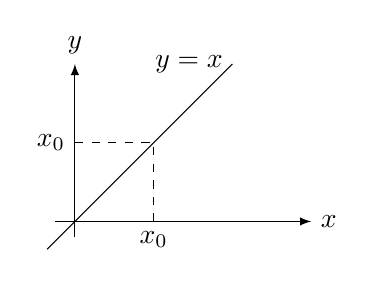
\begin{tikzpicture}
\draw[-latex](-0.25,0)--(3,0)node[right]{$x$};
\draw[-latex](0,-0.2)--(0,2)node[above]{$y$};
\draw[shorten <=-0.5cm](0,0)--(2,2)node[pos=1,left]{$y=x$};
\draw[dashed] (0,1)node[left]{$x_0$}--(1,1)--(1,0)node[below]{$x_0$};
\end{tikzpicture}
\caption{مماثل تفاعل}
\end{subfigure}%
\begin{subfigure}{0.5\textwidth}
\centering
\begin{tikzpicture}
\draw[-latex](-0.25,0)--(3,0)node[right]{$x$};
\draw[-latex](0,-0.2)--(0,2)node[above]{$y$};
\draw(-0.25,1)--(3,1)node[pos=0.9,above]{$y=k$};
\draw(0,1)node[circ]{}node[above left]{$k$};
\draw[dashed](1,0)node[below]{$x_0$}--(1,1)node[circ]{};
\draw(0,0)node[below left]{$M$};
\end{tikzpicture}
\caption{مستقل تفاعل}
\end{subfigure}%
\caption{اشکال برائے مثال \حوالہ{مثال_حد_عجیب_تفاعل_پ}}
\label{شکل_مثال_حد_عجیب_تفاعل_پ}
\end{figure}
\انتہا{مثال}
%==================================
\ابتدا{مثال}\شناخت{مثال_حد_عجیب_تفاعل_ت} \ترچھا{عین ممکن ہے کہ تفاعل کے دائرہ کار میں تفاعل کا حد نہ پایا جاتا ہو۔}\\ 
درج ذیل تفاعل کا \عددی{x\to 0} پر رویہ کیسا ہو گا؟
\begin{enumerate}[a.]
\item
$U(x)=\begin{cases}0,&x<0\\ 1,&x\ge 0  \end{cases}$
\item
$g(x)=\begin{cases} \tfrac{1}{x},&x\ne 0\\ 0,&x=0 \end{cases}$
\item
$f(x)=\begin{cases}0,&x\le 0\\ \sin \tfrac{1}{x},&x>0  \end{cases}$
\end{enumerate}
%

حل:\quad
\begin{enumerate}[a.]
\item
اکائی سیڑھی تفاعل \عددی{U(x)} کا \عددی{x\to 0} پر کوئی حد نہیں پایا جاتا ہے چونکہ اس نقطہ پر تفاعل کی چھلانگ پائی جاتی ہے۔\عددی{0} کے کافی قریب \عددی{x} کی منفی قیمتوں کے لئے \عددی{U} کی قیمت \عددی{0} ہے جبکہ \عددی{0} کے کافی  قریب  \عددی{x}  کی مثبت قیمتوں کے لئے \عددی{U} کی قیمت \عددی{1} ہے۔یوں \عددی{0} کے قریب پہنچنے سے \عددی{U} کی منفرد قیمت نہیں پائی جاتی ہے (شکل \حوالہ{شکل_مثال_حد_عجیب_تفاعل_ت}-ا)۔
\item
\عددی{x=0} کے کافی قریب تفاعل کی قیمت بے قابو بڑھتی ہے اور کسی ایک منفرد قیمت تک پہنچنے کی کوشش نہیں کرتی ہے (شکل \حوالہ{شکل_مثال_حد_عجیب_تفاعل_ت}-ب)۔
\item
\عددی{x=0} کے کافی قریب تفاعل بہت زیادہ ارتعاش کرتا ہے۔اس کی قیمت کسی مخصوص قیمت تک پہنچنے کی کوشش نہیں کرتی ہے (شکل \حوالہ{شکل_مثال_حد_عجیب_تفاعل_ت}-ج)۔ 
\end{enumerate}
%
\begin{figure}
\centering
\begin{subfigure}{0.33\textwidth}
\centering
\begin{tikzpicture}
\begin{axis}[clip=false,small,axis lines=middle,width=4cm,xtick={\empty},ytick={1},xlabel={$x$},ylabel={$y$},xlabel style={at={(current axis.right of origin)},anchor={west}},ylabel style={at={(current axis.above origin)},anchor=south},ymin=-0.5,ymax=2]
\addplot[domain=-2:0]{0};
\addplot[domain=0:2]{1};
\draw(axis cs:0,0)node[ocirc]{};
\draw(axis cs:0,1)node[circ]{};
\draw(axis cs:0,1)node[above right,font=\footnotesize]{$\begin{aligned}y=\begin{cases}0,&x<0\\ 1,&x\ge 1\end{cases}\end{aligned}$};
\end{axis}
\end{tikzpicture}
\caption{اکائی سیڑھی تفاعل $U(x)\,\,$}
\end{subfigure}%
\begin{subfigure}{0.33\textwidth}
\centering
\begin{tikzpicture}
\begin{axis}[clip=false,small,axis lines=middle,width=4cm,xtick={\empty},ytick={\empty},xlabel={$x$},ylabel={$y$},xlabel style={at={(current axis.right of origin)},anchor={west}},ylabel style={at={(current axis.above origin)},anchor=south}]
\addplot[domain=-4:-0.3]{1/x};
\addplot[domain=0.3:4]{1/x};
\draw(axis cs:0,0)node[circ]{}node[below right]{$0$};
\draw(axis cs:0.4,1)node[above right,font=\footnotesize]{$\begin{aligned}y=\begin{cases}\tfrac{1}{x},&x\ne 0\\ 0,&x=0\end{cases}\end{aligned}$};
\end{axis}
\end{tikzpicture}
\caption{$g(x)$}
\end{subfigure}%
\begin{subfigure}{0.33\textwidth}
\centering
\begin{tikzpicture}
\begin{axis}[clip=false,small,axis lines=middle,width=4cm,xtick={\empty},ytick={-1,1},xlabel={$x$},ylabel={$y$},xlabel style={at={(current axis.right of origin)},anchor={west}},ylabel style={at={(current axis.above origin)},anchor=south},ymin=-1.2,ymax=1.2]
\addplot[domain=-0.2:0]{0}node[circ]{};
\addplot[domain=0.052:0.08,samples=100]{sin(180/(pi*x)};
\addplot[domain=0.08:0.5,samples=100]{sin(180/(pi*x)};
\draw(axis cs:0,0)node[circ]{}node[below left]{$0$};
\draw(axis cs:0.2,-0.75)node[right,font=\footnotesize]{$\begin{aligned}y=\begin{cases}0 ,&x\le  0\\  \sin \tfrac{1}{x},&x>0\end{cases}\end{aligned}$};
\end{axis}
\end{tikzpicture}
\caption{$f(x)$}
\end{subfigure}%
\caption{اشکال برائے مثال \حوالہ{مثال_حد_عجیب_تفاعل_ت}}
\label{شکل_مثال_حد_عجیب_تفاعل_ت}
\end{figure}
\انتہا{مثال}
%=================================

\حصہء{سوالات}

\موٹا{ترسیم سے حد}\\
\ابتدا{سوال}\شناخت{سوال_حد_ترسیم_سے_حد_الف}
شکل \حوالہ{شکل_سوال_حد_ترسیم_سے_حد_الف}-ا میں دی گئی ترسیم سے درج ذیل حد تلاش کریں یا حد نا ہونے کی وجہ بیان کریں۔
\begin{multicols}{3}
\begin{enumerate}[a.]
\item
$\lim\limits_{x\to 1} g(x)$
\item
$\lim\limits_{x\to 2} g(x)$
\item
$\lim\limits_{x\to 3}g(x)$
\end{enumerate}
\end{multicols}
%
\begin{figure}
\centering
\begin{subfigure}{0.5\textwidth}
\centering
\begin{tikzpicture}
\draw[-latex](-0.25,0)--(4,0)node[right]{$x$};
\draw[-latex](0,-0.2)--(0,1.5)node[above]{$y$};
\draw[dashed](0,1)node[left]{$1$}--(3,1)node[solid,circ]{};
\draw(-0.2,-0.2)--(1,1)node[ocirc]{};
\draw(1,0)node[circ]{}--(2,1)node[circ]{}node[above,yshift={2mm}]{$y=g(x)$}--(3,0)node[ocirc]{}--(3.9,0.9);
\foreach \x in {1,2,3}{\draw(\x,0)node[below]{$\x$}--++(0,0.1);}
\end{tikzpicture}
\caption{}
\end{subfigure}%
\begin{subfigure}{0.5\textwidth}
\centering
\begin{tikzpicture}
\draw[-latex](-3,0)--(2,0)node[right]{$t$};
\draw[-latex](0,-1.25)--(0,1.5)node[above]{$s$};
\draw(-3,-1)--(-2,0)node[ocirc]{}node[above,yshift={2mm}]{$s=f(t)$}--(-1,-1)node[circ]{}--(0,-1)node[ocirc]{}node[right]{$-1$};
\foreach \x in {-2,-1,1}{\draw(\x,0)node[below]{$\x$}--++(0,0.1);}
\draw(0,0)node[circ]{}node[below left]{$0$};
\draw(0,1)node[ocirc]{}node[left]{$1$}--(2,1);
\end{tikzpicture}
\caption{}
\end{subfigure}%
\caption{اشکال برائے سوال \حوالہ{سوال_حد_ترسیم_سے_حد_الف} اور سوال \حوالہ{سوال_حد_ترسیم_سے_حد_ب}}
\label{شکل_سوال_حد_ترسیم_سے_حد_الف}
\end{figure}
\انتہا{سوال}
%=====================
\ابتدا{سوال}\شناخت{سوال_حد_ترسیم_سے_حد_ب}
شکل \حوالہ{شکل_سوال_حد_ترسیم_سے_حد_الف}-ب میں دی گئی ترسیم سے درج ذیل حد تلاش کریں یا حد نا ہونے کی وجہ بیان کریں۔
\begin{multicols}{3}
\begin{enumerate}[a.]
\item
$\lim\limits_{t\to -2}f(t)$
\item
$\lim\limits_{t\to -1}f(t)$
\item
$\lim\limits_{t\to 0}f(t)$
\end{enumerate}
\end{multicols}
\انتہا{سوال}
%======================
\ابتدا{سوال}\شناخت{سوال_حد_ترسیم_سے_حد_پ}
تفاعل \عددی{y=f(x)}  (شکل \حوالہ{سوال_حد_ترسیم_سے_حد_پ}-ا) کے لئے درج ذیل فقروں میں سے کون سے درست ہیں؟
\begin{multicols}{3}
\begin{enumerate}[a.]
\item
$\lim\limits_{x\to 0}f(x)$ موجود ہے\\
\item
$\lim\limits_{x\to 0}f(x)=0$
\item
$\lim\limits_{x\to 0}f(x)=1$
\item
$\lim\limits_{x\to 1}f(x)=1$
\item
$\lim\limits_{x\to 1}f(x)=0$
\item
$\lim\limits_{x\to x_ 0}f(x)$
وقفہ \عددی{(-1,1)} میں ہر نقطہ \عددی{x_0} پر موجود ہے
\end{enumerate}
\end{multicols}
%
\begin{figure}
\centering
\begin{subfigure}{0.5\textwidth}
\centering
\begin{tikzpicture}
\draw[-latex](-1.2,0)--(3,0)node[right]{$x$};
\draw[-latex](0,-1.2)--(0,1.5)node[above]{$y$};
\draw(-1,-1)node[circ]{}--(0,0)node[ocirc]{}--(1,-1)node[ocirc]{} (1,0)node[circ]{}--(2,1)node[circ]{};
\draw(0,1)node[circ]{}node[left]{$1$}--++(0.1,0);
\foreach \x in {-1,1,2}{\draw(\x,0)node[below]{$\x$}--++(0,0.1);} 
\draw(0,-1)node[left]{$-1$}--++(0.1,0);
\draw(0.5,1.25)node[right]{$y=f(x)$};
\end{tikzpicture}
\caption{}
\end{subfigure}%
\begin{subfigure}{0.5\textwidth}
\centering
\begin{tikzpicture}[]
\draw[-latex](-1.2,0)--(3.5,0)node[right]{$x$};
\draw[-latex](0,-2.2)--(0,1.5)node[above]{$y$};
\foreach \x in {-1,1,2,3}{\draw(\x,0)node[below]{$\x$}--++(0,0.1);} 
\foreach \y in {-2,-1,1}{\draw(0,\y)node[left]{$\y$}--++(0.1,0);}
\draw(-1,-1)node[circ]{}--(0,0)node[circ]{};
\draw[domain=0:1] plot ({\x},{-2*\x*\x});
\draw([shift={(0:1)}]2,0) arc (0:180:1);
\draw(1,0)node[circ]{} (2,0)node[circ]{} (3,0)node[circ]{} (2,1)node[ocirc]{}node[above]{$y=f(x)$};
\end{tikzpicture}
\caption{}
\end{subfigure}%
\caption{اشکال برائے سوال \حوالہ{سوال_حد_ترسیم_سے_حد_پ} اور سوال \حوالہ{سوال_حد_ترسیم_سے_حد_ت}}
\label{شکل_سوال_حد_ترسیم_سے_حد_پ}
\end{figure}
\انتہا{سوال}
%============================
\ابتدا{سوال}\شناخت{سوال_حد_ترسیم_سے_حد_ت}
تفاعل \عددی{y=f(x)} (شکل \حوالہ{سوال_حد_ترسیم_سے_حد_پ}-ب)  کے لئے درج ذیل فقروں میں سے کون سے درست ہیں؟
\begin{multicols}{3}
\begin{enumerate}[a.]
\item
$\lim\limits_{x\to 2} f(x)$
موجود نہیں ہے
\item
$\lim\limits_{x\to 2}f(x)=2$
\item
$\lim\limits_{x\to 1}f(x)$
موجود نہیں ہے
\item
$\lim\limits_{x\to x_0}f(x)$
وقفہ \عددی{(-1,1)} میں ہر نقطہ \عددی{x_0} پر موجود ہے۔
\item
$\lim\limits_{x\to x_0}f(x)$
وقفہ \عددی{(1,3)} میں ہر نقطہ \عددی{x_0} پر موجود ہے۔
\end{enumerate}
\end{multicols}
\انتہا{سوال}
%======================

\موٹا{وجودیت اور حد}\\
سوال \حوالہ{سوال_حد_غیر_موجود_الف} اور سوال \حوالہ{سوال_حد_غیر_موجود_ب} میں حد کی غیر موجودگی کی وجہ بیان کریں۔

\ابتدا{سوال}\شناخت{سوال_حد_غیر_موجود_الف}
$\lim\limits_{x \to 0}\tfrac{x}{\abs{x}}$
\انتہا{سوال}
%======================
\ابتدا{سوال}\شناخت{سوال_حد_غیر_موجود_ب}
$\lim\limits_{x \to 1}\tfrac{1}{x-1}$
\انتہا{سوال}
%======================
\ابتدا{سوال}
فرض کریں کہ ماسوائے نقطہ \عددی{x=x_0} تفاعل \عددی{f(x)} تمام حقیقی \عددی{x} کے لئے معین ہے۔کیا \عددی{\lim\limits_{x\to x_0}f(x)} کی وجودیت کی وجودیت کے بارے میں کچھ کہنا ممکن ہے؟ اپنے جواب کی وجہ بیان کریں۔ 
\انتہا{سوال}
%======================
\ابتدا{سوال}
فرض کریں کہ  تفاعل \عددی{f(x)} وقفہ \عددی{[-1,1]} میں تمام  \عددی{x} کے لئے معین ہے۔کیا \عددی{\lim\limits_{x\to 0}f(x)} کے بارے میں کچھ کہنا ممکن ہے؟ اپنے جواب کی وجہ بیان کریں۔ 
\انتہا{سوال}
%======================
\ابتدا{سوال}
اگر \عددی{\lim\limits_{x\to 1}f(x)=5} ہو تب کیا \عددی{x=1} پر \عددی{f} کا معین ہونا لازم ہے؟اگر معین ہونا لازم ہو تب کیا \عددی{f(1)=5} ہونا لازم ہے؟ کیا \عددی{x=1} پر ہم \عددی{f} کی قیمت کے بارے میں کچھ کہہ سکتے ہیں؟ وضاحت کریں۔
\انتہا{سوال}
%======================
\ابتدا{سوال}
اگر \عددی{f(1)=5} ہو تب کیا \عددی{\lim\limits_{x\to 1}f(x)} لازماً موجود ہو گا؟ اگر ایسا ہو تب کیا \عددی{\lim\limits_{x\to 1}f(x)=5} لازماً ہو گا؟ کیا ہم  \عددی{\lim\limits_{x\to 1}f(x)} کے بارے میں کوئی نتیجہ اخذ کر سکتے ہیں؟ وضاحت کریں۔
\انتہا{سوال}
%======================

\موٹا{کیلکولیٹر اور کمپیوٹر کا استعمال}\\

\ابتدا{سوال}
\عددی{f(x)=\tfrac{x^2-9}{x+3}} لیں۔
\begin{enumerate}[a.]
\item
\عددی{f} کی قیمتوں کا جدول نقاط \عددی{x=-3.1,-3.01,-3.001,\cdots} پر وہاں تک تلاش کریں جہاں تک آپ کا کیلکولیٹر جواب حاصل کر سکتا ہو۔اس جدول سے \عددی{\lim\limits_{x\to -3}f(x)} کی اندازاً قیمت حاصل کریں۔اس کے برعکس نقاط \عددی{x=-2.9,-2.99,-2.999,\cdots} پر \عددی{f} کی قیمتیں استعمال کرتے ہوئے نتیجہ کیا ہو گا؟
\item
تفاعل کو \عددی{x_0=-3} کے قریب ترسیم کریں۔ ترسیم پر \عددی{x\to -3} کے لئے \عددی{y} کی قیمت دیکھ کر  گزشتہ جزو کے نتائج کی تصدیق کریں۔ 
\item
\عددی{\lim\limits_{x\to -3}f(x)} کو الجبرائی طریقہ سے اخذ کریں۔
\end{enumerate}
\انتہا{سوال}
%=========================
\ابتدا{سوال}
\عددی{g(x)=\tfrac{x^2-2}{x-\sqrt{2}}} لیں۔
\begin{enumerate}[a.]
\item
\عددی{\sqrt{2}} کی تخمینی قیمتوں \عددی{x=1.4,1.41,1.414,\cdots} پر تفاعل کی قیمتوں کے جدول سے \عددی{\lim\limits_{x\to \sqrt{2}}g(x)}  کی اندازاً قیمت حاصل کریں۔
\item
نقطہ \عددی{x_0=\sqrt{2}} کے قریب تفاعل ترسیم کریں۔\عددی{x\to \sqrt{2}} کے لئے ترسیم سے \عددی{y} کی قیمت دیکھ کر گزشتہ جزو کی جواب کا تصدیق کریں۔
\item
\عددی{\lim\limits_{x\to\sqrt{2}}g(x)} کو الجبرائی طور پر حاصل کریں۔
\end{enumerate}
\انتہا{سوال}
%====================
\ابتدا{سوال}
\عددی{G(x)=\tfrac{x+6}{x^2+4x-12}} لیں۔
\begin{enumerate}[a.]
\item
نقاط \عددی{x=-5.9,-5.99,-5.999,\cdots} پر \عددی{G} کی قیمتوں کا جدول بنا کر \عددی{\lim\limits_{x\to -6}G(x)} کی اندازاً قیمت حاصل کریں۔ اس کے برعکس \عددی{x=-6.1,-6.01,-6.001,\cdots} پر \عددی{G} کی قیمتیں استعمال کرتے ہوئے کیا نتیجہ حاصل ہو گا؟
\item
\عددی{G} کو \عددی{x_0=6} کے قریبی نقطوں پر تقسیم کرتے ہوئے \عددی{x\to -6} کے لئے \عددی{G} کی قیمت دیکھ کر گزشتہ جزو کے نتائج کی تصدیق کریں۔
\item
\عددی{\lim\limits_{x\to -6}G(x)} کو الجبرائی طریقہ سے حاصل کریں۔
\end{enumerate}
\انتہا{سوال}
%======================
\ابتدا{سوال}
\عددی{h(x)=\tfrac{x^2-2x-3}{x^2-4x+3}} لیں۔
\begin{enumerate}[a.]
\item
نقاط \عددی{x=2.9, 2.99, 2.999,\cdots} پر \عددی{h} کی قیمتوں کے جدول سے \عددی{\lim\limits_{x\to 3}h(x)} کی اندازاً قیمت تلاش کریں۔اس کے برعکس \عددی{x=3.1,3.01,3.001,\cdots} پر \عددی{h} کی قیمتیں لیتے ہوئے نتیجہ کیا ہو گا؟
\item
\عددی{x_0=3} کے قریب \عددی{h} ترسیم کر کے \عددی{x\to 3} کے لئے \عددی{h(x)} کی قیمت دیکھ کر گزشتہ جزو کے نتائج کی تصدیق کریں۔
\item
\عددی{\lim\limits_{x\to 3}h(x)} کو الجبرائی طریقہ سے حاصل کریں۔
\end{enumerate}
\انتہا{سوال}
%=====================
\ابتدا{سوال}
\عددی{f(x)=\tfrac{x^2-1}{\abs{x}-1}} لیں۔
\begin{enumerate}[a.]
\item
\عددی{f} کی قیمتوں کا جدول \عددی{x} کی ان قیمتوں کے لئے بنائیں جو \عددی{x_0=-1} تک نیچے سے اور اوپر سے پہنچنے کی کوشش کرتی ہیں۔اس جدول سے \عددی{\lim\limits_{x\to-1}f(x)} کی اندازاً قیمت تلاش کریں۔  
\item
\عددی{x_0=-1} کے قریب \عددی{f} ترسیم کریں۔ترسیم سے \عددی{x\to -1} کے لئے \عددی{y} کی قیمتیں دیکھ کر گزشتہ جزو کے نتائج کی تصدیق کریں۔
\item
\عددی{\lim\limits_{x\to -1}f(x)} کو الجبرائی طریقہ سے حاصل کریں۔
\end{enumerate}
\انتہا{سوال}
%========================
\ابتدا{سوال}
\عددی{F(x)=\tfrac{x^2+3x+2}{2-\abs{x}}} لیں۔
\begin{enumerate}[a.]
\item
\عددی{F} کی قیمتوں کا جدول \عددی{x} کی ان قیمتوں کے لئے بنائیں جو \عددی{x_0=-2} تک نیچے سے اور اوپر سے پہنچنے کی کوشش کرتی ہیں۔اس جدول سے
 \عددی{\lim\limits_{x\to-2}F(x)} کی اندازاً قیمت تلاش کریں۔  
\item
\عددی{x_0=-2} کے قریب \عددی{F} ترسیم کریں۔ترسیم سے \عددی{x\to -2} کے لئے \عددی{y} کی قیمتیں دیکھ کر گزشتہ جزو کے نتائج کی تصدیق کریں۔
\item
\عددی{\lim\limits_{x\to -2}F(x)} کو الجبرائی طریقہ سے حاصل کریں۔
\end{enumerate}
\انتہا{سوال}
%========================
\ابتدا{سوال}
\عددی{g(\theta)=\tfrac{\sin\theta}{\theta}} لیں۔
\begin{enumerate}[a.]
\item
\عددی{g} کی قیمتوں کا جدول \عددی{\theta} کی ان قیمتوں کے لئے بنائیں جو \عددی{\theta_0=0} تک نیچے سے اور اوپر سے پہنچنے کی کوشش کرتی ہیں۔اس جدول سے
 \عددی{\lim\limits_{x\to 0}g(\theta)} کی اندازاً قیمت تلاش کریں۔  
\item
\عددی{\theta_0=0} کے قریب \عددی{g} ترسیم کریں۔ترسیم سے گزشتہ جزو کے نتائج کی تصدیق کریں۔
\end{enumerate}
\انتہا{سوال}
%========================
\ابتدا{سوال}
\عددی{G(t)=\tfrac{1-\cos t}{t^2}} لیں۔
\begin{enumerate}[a.]
\item
\عددی{G} کی قیمتوں کا جدول \عددی{t} کی ان قیمتوں کے لئے بنائیں جو \عددی{t_0=0} تک نیچے سے اور اوپر سے پہنچنے کی کوشش کرتی ہیں۔اس جدول سے
 \عددی{\lim\limits_{t\to 0}G(t)} کی اندازاً قیمت تلاش کریں۔  
\item
\عددی{t_0=0} کے قریب \عددی{G} ترسیم کریں۔ترسیم سے گزشتہ جزو کے نتائج کی تصدیق کریں۔
\end{enumerate}
\انتہا{سوال}
%===================
\ابتدا{سوال}
\عددی{f(x)=x^{\tfrac{1}{1-x}}} لیں۔
\begin{enumerate}[a.]
\item
\عددی{f} کی قیمتوں کا جدول \عددی{x} کی ان قیمتوں کے لئے بنائیں جو \عددی{x_0=1} تک نیچے سے اور اوپر سے پہنچنے کی کوشش کرتی ہیں۔کیا \عددی{x} کی قیمت \عددی{x\to 1} تک پہنچنے سے \عددی{f} کا تحدیدی نقطہ پایا جاتا ہے؟ اگر تحدیدی نقطہ پایا جاتا ہو، اس کا تلاش کریں۔اگر نہیں پایا جاتا ہو تب وجہ بیان کریں۔
\item
\عددی{x_0=1} کے قریب \عددی{f} ترسیم کریں۔ترسیم سے گزشتہ جزو کے نتائج کی تصدیق کریں۔
\end{enumerate}
\انتہا{سوال}
%=============================
\ابتدا{سوال}
\عددی{f(x)=\tfrac{3^x-1}{x}} لیں۔
\begin{enumerate}[a.]
\item
\عددی{f} کی قیمتوں کا جدول \عددی{x} کی ان قیمتوں کے لئے بنائیں جو \عددی{x_0=0} تک نیچے سے اور اوپر سے پہنچنے کی کوشش کرتی ہیں۔کیا
 \عددی{x} کی قیمت \عددی{x\to 0} تک پہنچنے سے \عددی{f} کا تحدیدی نقطہ پایا جاتا ہے؟ اگر تحدیدی نقطہ پایا جاتا ہو، اس کا تلاش کریں۔اگر نہیں پایا جاتا ہو تب وجہ بیان کریں۔
\item
\عددی{x_0=0} کے قریب \عددی{f} ترسیم کریں۔ترسیم سے گزشتہ جزو کے نتائج کی تصدیق کریں۔
\end{enumerate}
\انتہا{سوال}
%=============================
\موٹا{متغیر کی تحدیدی قیمت پر کرتے ہوئے حد کا تعین}\\
سوال \حوالہ{سوال_حد_پر_الف} تا سوال \حوالہ{سوال_حد_پر_ب} میں متغیر \عددی{x} کی تحدیدی قیمت کو تفاعل میں پر کرتے ہوئے تفاعل کی حد تلاش کریں۔

\ابتدا{سوال}\شناخت{سوال_حد_پر_الف}
$\lim\limits_{x\to 2} 2x$
\انتہا{سوال}
%========================
\ابتدا{سوال}
$\lim\limits_{x\to 0} 2x$
\انتہا{سوال}
%========================
\ابتدا{سوال}
$\lim\limits_{x\to \tfrac{1}{3}} (3x-1)$
\انتہا{سوال}
%========================
\ابتدا{سوال}
$\lim\limits_{x\to 1} -\tfrac{1}{3x-1}$
\انتہا{سوال}
%========================
\ابتدا{سوال}
$\lim\limits_{x\to -1} 3x(2x-1)$
\انتہا{سوال}
%========================
\ابتدا{سوال}
$\lim\limits_{x\to -1} \tfrac{3x^2}{2x-1}$
\انتہا{سوال}
%========================
\ابتدا{سوال}
$\lim\limits_{x\to \tfrac{\pi}{2}} x\sin x$
\انتہا{سوال}
%========================
\ابتدا{سوال}\شناخت{سوال_حد_پر_ب}
$\lim\limits_{x\to \pi} \tfrac{\cos x}{1-\pi}$
\انتہا{سوال}
%========================

\موٹا{اوسط شرح تبدیلی}\\
سوال \حوالہ{سوال_حد_اوسط_تبدیلی_شرح_الف} تا سوال \حوالہ{سوال_حد_اوسط_تبدیلی_شرح_ب} میں دیے وقفہ پر تفاعل کی اوسط شرح تبدیلی تلاش کریں۔

\ابتدا{سوال}\شناخت{سوال_حد_اوسط_تبدیلی_شرح_الف}
\عددی{f(x)=x^3+1}؛ (الف) \عددی{[2,3]}، (ب) \عددی{[-1,1]}
\انتہا{سوال}
%======================
\ابتدا{سوال}
\عددی{g(x)=x^2}؛ (الف) \عددی{[-1,1]}، (ب) \عددی{[-2,0]}
\انتہا{سوال}
%======================
\ابتدا{سوال}
\عددی{h(t)=\cos t}؛ (الف) \عددی{[\tfrac{\pi}{4},\tfrac{3\pi}{4}]}، (ب) \عددی{[\tfrac{\pi}{6},\tfrac{\pi}{2}]}
\انتہا{سوال}
%======================
\ابتدا{سوال}
\عددی{g(t)=2+\cos t}؛ (الف) \عددی{[0,\pi]}، (ب) \عددی{[-\pi,\pi]}
\انتہا{سوال}
%======================
\ابتدا{سوال}
\عددی{R(\theta)=\sqrt{4\theta+1}}؛  \عددی{[0,2]}
\انتہا{سوال}
%======================
\ابتدا{سوال}\شناخت{سوال_حد_اوسط_تبدیلی_شرح_ب}
\عددی{P(\theta)=\theta^3-4\theta^2+5\theta}؛  \عددی{[1,2]}
\انتہا{سوال}
%======================
\ابتدا{سوال}\شناخت{سوال_حد_چاند_الف}
چاند پر ساکن حالت سے گرنے والی چیز کا فاصلہ بالمقابل وقت ترسیم شکل \حوالہ{شکل_سوال_حد_چاند_الف} میں دکھایا گیا ہے۔ (الف) سیکنٹ \عددی{NQ_1}، \عددی{NQ_2}، \نقطے \عددی{NQ_6} کی اندازاً ڈھلوان تلاش کر کے جدول میں لکھیں۔ (ب) اس جدول سے \عددی{t=\SI{10}{\second}} پر رفتار کی اندازاً قیمت حاصل کریں۔
\begin{figure}
\centering
\begin{tikzpicture}
\begin{axis}[clip=false,small,axis lines=middle,grid=both,xlabel={ (سیکنڈ)$t$},ylabel={(میٹر)$y$}]
\addplot[domain=0:10]{1/2*1.6*x^2}node[circ]{}node[right]{$N$};
\draw(axis cs:5,20)node[circ]{}node[right]{$Q_1$};
\draw(axis cs:6,28.8)node[circ]{}node[right]{$Q_2$};
\draw(axis cs:7.07,40)node[circ]{}node[right]{$Q_3$};
\draw(axis cs:8,51.2)node[circ]{}node[right]{$Q_4$};
\draw(axis cs:8.66,60)node[circ]{}node[right]{$Q_5$};
\draw(axis cs:9.35,70)node[circ]{}node[right]{$Q_6$};
\end{axis}
\end{tikzpicture}
\caption{چاند پر ساکن حالت سے گرنے والی چیز کا فاصلہ بالمقابل وقت ترسیم}
\label{شکل_سوال_حد_چاند_الف}
\end{figure}
\انتہا{سوال}
%==================
\ابتدا{سوال}
ایک چھوٹی کمپنی کے پہلے چار سال کا منافع درج ذیل ہے۔(الف) منافع بالمقابل سال کو بطور نقطے ترسیم کرتے ہوئے انہیں ہموار ترین لکیر سے ملائیں۔ (ب)  \عددی{1992} اور \عددی{1994} کے بیچ منافع بڑھنے کی اوسط شرح تلاش کریں۔ (پ) ترسیم استعمال کرتے ہوئے \عددی{1992} کے دوران منافع بڑھنے کی شرح تلاش کریں۔
\begin{align*}
\begin{array}{rr}
\multicolumn{1}{c}{\text{سال}}&\multicolumn{1}{c}{\text{\RL{منافع (لاکھ)}}}\\
\hline
1990&6\\
1991&27\\
1992&62\\
1993&111\\
1994&174
\end{array}
\end{align*}
\انتہا{سوال}
%==========================
\ابتدا{سوال}
تفاعل \عددی{F(x)=\tfrac{x+2}{x-2}} کی قیمتیں نقطہ \عددی{x=2}، \عددی{\tfrac{11}{10}}، \عددی{\tfrac{101}{100}}، \عددی{\tfrac{1001}{1000}}، \عددی{\tfrac{10001}{10000}} اور \عددی{x=1} پر  حاصل کر کے جدول میں لکھیں۔(الف) جدول میں پائے جانے والے ہر \عددی{x\ne 1} کے لئے وقفہ \عددی{[1,x]} پر تفاعل کی اوسط شرح تبدیلی حاصل کریں۔ (ب) \عددی{x=1} پر \عددی{F(x)} کی شرح تبدیلی تلاش کریں۔اگر جدول بڑھانے کی ضرورت ہو تو جدول بڑھائیں۔ 
\انتہا{سوال}
%===========================
\ابتدا{سوال}
\عددی{x\ge 0} کے لئے \عددی{g(x)=\sqrt{x}} لیں۔
\begin{enumerate}[a.]
\item
وقفہ \عددی{[1,2]}، \عددی{[1,1.5]} اور \عددی{[1,1+h]} پر \عددی{x} کے  لحاظ سے \عددی{g(x)} کی اوسط شرح تبدیلی تلاش کریں۔
\item
صفر کے قریب \عددی{h} کی قیمتوں، مثلاً \عددی{h=0.1,0.01,0.001,0.0001,0.00001} کے لئے \عددی{x} کے لحاظ سے وقفہ \عددی{[1,1+h]} پر \عددی{g(x)} کی اوسط شرح تبدیلی تلاش کریں۔
\item
جدول سے \عددی{x=1} پر \عددی{g(x)} کی تبدیلی کی شرح کیا ہے؟
\item
\عددی{h\to 0} کے لئے \عددی{g(x)} کی تبدیلی کی شرح الجبرائی طریقہ سے حاصل کریں۔
\end{enumerate}
\انتہا{سوال}
%======================
\ابتدا{سوال}
\عددی{t\ne 0} کے لئے \عددی{f(t)=\tfrac{1}{t}} لیں۔
\begin{enumerate}[a.]
\item
(الف) وقفہ \عددی{t=2} تا \عددی{t=3} اور  (ب) وقفہ \عددی{t=2} تا \عددی{t=T} پر \عددی{t} کے لحاظ سے \عددی{g(t)} کی اوسط شرح تبدیلی تلاش کریں۔ 
\item
\عددی{2} تک پہنچنے والی \عددی{T} کی قیمتوں، مثلاً \عددی{T=2.1}، \عددی{T=2.01}، \عددی{T=2.001}، \عددی{T=2.0001}، \عددی{T=2.00001} اور \عددی{T=2.000001}، کے لئے وقفہ \عددی{[2,T]} پر \عددی{t} کے لحاظ سے \عددی{f(t)} کی اوسط شرح تبدیلی تلاش کر کر جدول میں لکھیں۔
\item
اس جدول سے \عددی{t=2} پر \عددی{t} کے لحاظ سے \عددی{f} کی شرح تبدیلی کیا ہے۔
\item
وقفہ \عددی{[2,T]} پر \عددی{t} کے لحاظ سے \عددی{f} کی شرح تبدیلی کی حد \عددی{T\to 2} کے لئے  تلاش کریں۔(\عددی{T=2} پر کرنے سے پہلے آپ کو کچھ الجبرا کرنا ہو گا۔)
\end{enumerate}
\انتہا{سوال}
%======================
سوال \حوالہ{سوال_حد_الجبرا_الف} تا سوال \حوالہ{سوال_حد_الجبرا_ب} کو کمپیوٹر کی مدد سے حل کریں۔(الف) نقطہ \عددی{x_0} کے قریب تفاعل ترسیم کریں۔ (ب) ترسیم کو دیکھ کر تفاعل کی حد کی اندازاً قیمت تلاش کریں۔ (پ) حد کو الجبرائی طور پر حاصل کریں۔

\ابتدا{سوال}\شناخت{سوال_حد_الجبرا_الف}
$\lim\limits_{x\to 2} \tfrac{x^4-16}{x-2}$
\انتہا{سوال}
%=========================
\ابتدا{سوال}
$\lim\limits_{x\to -1} \tfrac{x^3-x^2-5x-3}{(x+1)^2}$
\انتہا{سوال}
%=========================
\ابتدا{سوال}
$\lim\limits_{x\to 0} \tfrac{\sqrt[\leftroot{-2}3]{1+x}-1}{x}$
\انتہا{سوال}
%=========================
\ابتدا{سوال}
$\lim\limits_{x\to 3} \tfrac{x^2-9}{\sqrt{x^2+7}-4}$
\انتہا{سوال}
%=========================
\ابتدا{سوال}
$\lim\limits_{x\to 0} \tfrac{1-\cos x}{x\sin x}$
\انتہا{سوال}
%=========================
\ابتدا{سوال}\شناخت{سوال_حد_الجبرا_ب}
$\lim\limits_{x\to 0} \tfrac{2x^2}{3-3\cos x}$
\انتہا{سوال}
%=========================

\حصہ{حد تلاش کرنے کے قواعد}
حد تلاش کرنے کے مسئلوں کو اس حصہ میں پیش کیا جائے گا۔پہلے تین مسئلے مثال \حوالہ{مثال_حد_مماثل_تفاعل} کے نتائج کو لے کر کثیر رکنی، ناطق تفاعل اور طاقتوں  کے حد تلاش کرنے میں ہمیں مدد دیتے ہیں۔چوتھا مسئلہ بعد میں استعمال ہونے والی حساب کے لئے ہمیں تیار کرتا ہے۔

\جزوحصہء{طاقتوں اور الجبرائی مجموعوں کے حد}

\ابتدا{مسئلہ}\شناخت{مسئلہ_حد_قواعد-الف}\موٹا{حد کے خواص}\\
اگر \عددی{\lim\limits_{x\to c}f(x)=L} اور \عددی{\lim\limits_{x\to c}g(x)=M} ہوں،جہاں \عددی{L} اور \عددی{M} حقیقی اعداد ہیں،  تب درج ذیل قواعد مطمئن ہوں گے۔
\begin{description}
\item{قاعدہ مجموعہ:}\quad 
$\lim\limits_{x\to c}[f(x)+g(x)]=L+M$
\item{قاعدہ فرق:}\quad
$\lim\limits_{x\to c}[f(x)-g(x)]=L-M$
\item{قاعدہ ضرب:}\quad
$\lim\limits_{x\to c}[f(x)\cdot g(x)]=L\cdot M$
\item{قاعدہ ضرب مستقل:}\quad
$\lim\limits_{x\to c} k f(x)=kL$
\quad
(\عددی{k} مستقل عدد ہے)
\item{قاعدہ حاصل تقسیم:}\quad
$\lim\limits_{x\to c}\tfrac{f(x)}{g(x)}=\tfrac{L}{M}$
\quad
$M\ne 0$
\item{قاعدہ طاقت:}\quad
اگر \عددی{m} اور \عددی{n} عدد صحیح ہوں تب
$\lim\limits_{x\to c}[f(x)]^{\tfrac{m}{n}}=L^{\tfrac{m}{n}}$
 ہو گا بشرطیکہ  \عددی{L^{\tfrac{m}{n}}} حقیقی عدد ہو۔
\end{description}
\انتہا{مسئلہ}
%============================

الفاظ میں درج بالا مسئلہ درج ذیل کہتا ہے۔
\begin{enumerate}
\item
دو تفاعل کے مجموعے کا حد ان تفاعل کے انفرادی حدوں کا مجموعہ ہو گا۔
\item
دو تفاعل کے فرق  کا حد ان تفاعل کے انفرادی حدوں کا فرق ہو گا۔
\item
دو تفاعل کے حاصل ضرب  کا حد ان تفاعل کے انفرادی حدوں کا حاصل ضرب  ہو گا۔
\item
ایک تفاعل ضرب مستقل کا حد اس تفاعل کے حد ضرب مستقل ہو گا۔
\item
دو تفاعل کے حاصل تقسیم کا حد ان تفاعل کے انفرادی حدوں کا حاصل تقسیم ہو گا بشرطیکہ نسب نما تفاعل کا حد غیر صفر ہو۔
\item
تفاعل کے ناطق طاقت کا حد اس تفاعل کے حد کا ناطق طاقت ہو گا بشرطیکہ حد کا ناطق طاقت  حقیقی عدد ہو۔ 
\end{enumerate}

%===================
\ابتدا{مثال}\شناخت{مثال_حد_لمبا_تفاعل_الف}
\عددی{\lim\limits_{x\to c}\tfrac{x^3+4x^2-3}{x^2+5}} تلاش کریں۔\\
حل:\quad
مثال \حوالہ{مثال_حد_مماثل_تفاعل} کے نتائج \عددی{\lim\limits_{x\to c}x=c} اور \عددی{\lim\limits_{x\to c}k=k}  سے شروع کرتے ہوئے
 مسئلہ \حوالہ{مسئلہ_حد_قواعد-الف} کے مختلف شق استعمال کرتے ہوئے درج ذیل ملتا ہے۔

\begin{enumerate}[a.]
\item 
$\lim\limits_{x\to c} x^2=(\lim\limits_{x\to c} x)(\lim\limits_{x\to c}x)=c\cdot c=c^2$ \hfill 
حاصل ضرب یا طاقت
\item
$\lim\limits_{x\to c}(x^2+5)=\lim\limits_{x\to c}x^2+\lim\limits_{x\to c} 5=c^2+5$ \hfill
مجموعہ اور (ا)
\item
$\lim\limits_{x\to c} 4x^2=4\lim\limits_{x\to c}x^2=4c^2$\hfill
ضرب مستقل اور (ا) 
\item
$\lim\limits_{x\to c}(4x^2-3)=\lim\limits_{x\to c}4x^2-\lim\limits_{x\to c} 3=4c^2-3$ \hfill
فرق اور (ج)
\item
$\lim\limits_{x\to c}x^3=(\lim\limits_{x\to c}x^2)(\lim\limits_{x\to c} x)=c^2\cdot c=c^3$\hfill
حاصل ضرب اور (ا) یا طاقت
\item
$\lim\limits_{x\to c}(x^3+4x-3)=\lim\limits_{x\to c}x^3+\lim\limits_{x\to c}(4x^2-3)=c^3+4c^2-3$\hfill
  مجموعہ، (ج) اور (د)
\item
$\lim\limits_{x\to c}\tfrac{x^3+4x^2-3}{x^2+5}=\tfrac{\lim\limits_{x\to c}(x^3+4x^2-3)}{\lim\limits_{x\to c}(x^2+5)}=\tfrac{c^3+4c^2-3}{c^2+5}$\hfill
حاصل تقسیم، (ہ) اور (ب) 
\end{enumerate}
\انتہا{مثال}
%===================
\ابتدا{مثال}
\عددی{\lim\limits_{x\to -2}\sqrt{4x^2-3}} تلاش کریں۔\\
حل:\quad
\begin{align*}
\lim\limits_{x\to -2}\sqrt{4x^2-3}&=\sqrt{4(-2)^2-3}\quad\quad\quad  \text{\RL{مثال \حوالہ{مثال_حد_لمبا_تفاعل_الف}-د اور $n=\tfrac{1}{2}$ کے ساتھ قاعدہ طاقت}}\\
&=\sqrt{16-3}=\sqrt{13}
\end{align*}
\انتہا{مثال}
%=======================

مسئلہ \حوالہ{مسئلہ_حد_قواعد-الف} کے دو نتائج  کثیر رکنی اور ناطق تفاعل کا حد تلاش کرنے کو مزید آسان بناتے ہیں۔ \عددی{x\to c} کے لئے کثیر رکنی کا حد تلاش کرنے کی خاطر محض تفاعل کے کلیہ میں \عددی{x} کی جگہ \عددی{c} پر کریں۔ناطق تفاعل کا حد \عددی{x\to c} پر تلاش کرنے کی خاطر تفاعل کے کلیہ میں \عددی{x} کی جگہ \عددی{c} پر کریں بشرطیکہ نسب نما اس نقطہ پر غیر صفر ہو۔

\ابتدا{مسئلہ}\شناخت{مسئلہ_حد_قواعد_ب}\موٹا{کثیر رکنی کا حد متغیر میں مستقل پر کرنے سے حاصل ہو گا}\\
اگر \عددی{P(x)=a_nx^n+a_{n-1}x^{n-1}+\cdots+a_0} ہو تب درج ذیل ہو گا۔
\begin{align*}
\lim\limits_{x\to c} P(x)=P(c)=a_nc^n+a_{n-1}c^{n-1}+\cdots+a_0
\end{align*}
\انتہا{مسئلہ}
%==============================
\ابتدا{مسئلہ}\شناخت{مسئلہ_حد_قواعد_پ}\موٹا{غیر صفر نسب نما کی صورت میں ناطق تفاعل کا حد کلیہ میں متغیر کی جگہ مستقل پر کرنے سے حاصل ہو گا}\\
فرض کریں کہ \عددی{P(x)} اور \عددی{Q(x)} کثیر رکنی ہیں اور \عددی{Q(c)\ne 0} ہے تب درج ذیل ہو گا۔
\begin{align*}
\lim\limits_{x\to c} \frac{P(x)}{Q(x)}=\frac{P(c)}{Q(c)}
\end{align*}
\انتہا{مسئلہ}
%============================

\ابتدا{مثال}
\begin{align*}
\lim_{x\to -1}\frac{x^3+4x^2-3}{x^2+5}=\frac{(-1)^3+4(-1)^2-3}{(-1)^2+5}=\frac{0}{6}=0
\end{align*}
یہ ایک ہی قدم میں مثال \حوالہ{مثال_حد_لمبا_تفاعل_الف} کا حل ہے۔
\انتہا{مثال}
%========================

\جزوحصہء{صفر نسب نما کا الجبرائی طریقہ سے اسقاط}
مسئلہ \حوالہ{مسئلہ_حد_قواعد_پ} ناطق تفاعل پر صرف اس صورت قابل اطلاق ہے جب تحدیدی نقطہ  \عددی{c} پر تفاعل کا نسب نما غیر صفر ہو۔صفر نسب نما کی صورت میں بعض اوقات نسب نما اور شمار کنندہ میں یکساں اجزاء  کو منسوخ کرتے ہوئے  \عددی{c} پر غیر صفر نسب نما حاصل کیا جا سکتا ہے۔اگر ایسا ممکن ہو تب \عددی{x} کی جگہ \عددی{c} پر کرنے سے حد حاصل کیا جا سکتا ہے۔

\ابتدا{مثال}\شناخت{مثال_حد_اجزاء_منسوخ_الف}\ترچھا{یکساں جزو کی منسوخی}\\
\عددی{\lim\limits_{x\to 1}\tfrac{x^2+x-2}{x^2-x}} تلاش کریں۔\\
حل:\quad
ہم \عددی{x=1} پر نہیں کر سکتے ہیں چونکہ ایسا کرنے سے صفر نسب نما حاصل ہو گا اور صفر سے کسی بھی عدد کو تقسیم نہیں کیا جا سکتا ہے۔البتہ ہم نسب نما اور شمار کنندہ کو اجزاء ضربی کی صورت میں لکھ کر یکساں اجزاء کو آپس میں منسوخ کر سکتے ہیں۔
\begin{align*}
\frac{x^2+x-2}{x^2-x}&=\frac{(x-1)(x+2)}{x(x-1)}=\frac{x+2}{x}
\end{align*}
اب \عددی{x\ne 0} کی صورت میں  درج بالا کو حد تلاش کرنے کے لئے  استعمال کیا جا سکتا ہے۔یوں درج ذیل حاصل ہوتا ہے۔
\begin{align*}
\lim_{x \to 1} \frac{x^2+x-2}{x^2-x}=\lim_{x\to 1}\frac{x+2}{x}=\frac{1+2}{1}=3
\end{align*}
شکل \حوالہ{شکل_مثال_حد_اجزاء_منسوخ_الف} میں \عددی{y=\tfrac{x^2+x-2}{x^2-x}} اور \عددی{y=\tfrac{x+2}{x}} کے ترسیم دکھائے گئے ہیں۔یہ ترسیم صرف نقطہ \عددی{(1,3)} پر ایک دوسرے سے مختلف ہیں۔البتہ اس نقطہ پر دونوں تفاعل کا حد ایک جیسا ہے۔ 
%
\begin{figure}
\centering
\begin{subfigure}{0.5\textwidth}
\centering
\begin{tikzpicture}
\begin{axis}[small,axis lines=middle,xtick={-2,1},ytick={3},xlabel={$x$},ylabel={$y$},ylabel style={at={(current axis.above origin)},anchor=south}]
\addplot[domain=-4:-0.5]{(x+2)/x};
\addplot[domain=0.5:4]{(x+2)/x}node[pos=0.1,right]{$y=\frac{x^2+x-2}{x^2-x}$};
\draw(axis cs:1,3)node[ocirc]{}node[right]{$(1,3)$};
\end{axis}
\end{tikzpicture}
\caption{}
\end{subfigure}%
\begin{subfigure}{0.5\textwidth}
\centering
\begin{tikzpicture}
\begin{axis}[small,axis lines=middle,xtick={-2,1},ytick={3},xlabel={$x$},ylabel={$y$},ylabel style={at={(current axis.above origin)},anchor=south}]
\addplot[domain=-4:-0.5]{(x+2)/x};
\addplot[domain=0.5:4]{(x+2)/x}node[pos=0.1,right]{$y=\frac{x+2}{x}$};
\draw(axis cs:1,3)node[circ]{}node[right]{$(1,3)$};
\end{axis}
\end{tikzpicture}
\caption{}
\end{subfigure}%
\caption{ماسوائے نقطہ $(1,3)$ کے دونوں ترسیم یکساں ہیں}
\label{شکل_مثال_حد_اجزاء_منسوخ_الف}
\end{figure}
\انتہا{مثال}
%=====================
\ابتدا{مثال}\موٹا{ایک جیسے اجزاء پیدا کرتے ہوئے انہیں آپس میں منسوخ کرنا}\\
\عددی{\lim\limits_{h\to 0}\tfrac{\sqrt{2+h}-\sqrt{2}}{h}} تلاش کریں۔
\انتہا{مثال}
%=====================
